\documentclass{article}

\usepackage[utf8]{inputenc}
\usepackage{longtable}
\usepackage{authblk}
\usepackage{adjustbox}

\usepackage{natbib}



\title{CARACTERIZACIÓN DE LOS INDICES DE DESARROLLO HUMANO EN COLOMBIA}
% autores
\renewcommand\Authand{, y }
\author[1]{\normalsize Andrea Calderon Corredor}


\affil[1]{\small  Facultad de Ingeniería,Universidad de los Andes\\
\texttt{{a.calderon}@uniandes.edu.co}}
\affil[1]{\small Herramientas Computacionales para la Investigacion\\}


\date{29 de Junio de 2018}



%%%%%%%%%%%%%%%%%%%%%%%%%%%%%%%%%%%INICIO%CONTENIDO%%%%%%%%%%%%%%%%%%%%%%%%%%%%%%



\usepackage{Sweave}
\begin{document}
\Sconcordance{concordance:Preliminar.tex:Preliminar.Rnw:%
1 30 1 1 0 6 1 1 9 10 0 1 2 4 1 1 3 15 0 1 7 6 1 1 11 1 3 7 1 1 13 1 2 %
8 1}


\maketitle



\begin{Schunk}
\begin{Soutput}
'data.frame':	32 obs. of  6 variables:
 $ IDH               : num  0.879 0.867 0.865 0.849 0.842 0.839 0.837 0.835 0.834 0.832 ...
 $ Departamento      : chr  "Santander" "Casanare" "Valle del Cauca" "Antioquia" ...
 $ Poblacion.Cabecera: int  1587972 281548 4169553 5262172 742812 761658 10070801 2438533 56487 506254 ...
 $ Poblacion.Resto   : int  502867 93701 586560 1428858 539251 206109 914484 107391 21926 68756 ...
 $ Poblacion.Total   : int  2090839 375249 4756113 6691030 1282063 967767 10985285 2545924 78413 575010 ...
 $ DepartamentoNorm  : chr  "Santander" "Casanare" "Valle del Cauca" "Antioquia" ...
\end{Soutput}
\end{Schunk}

\section{Exploración Univariada}\label{univariada}

Teniendo en cuenta queel estudio se hizo para los 32 departamentos de Colombia

% Table created by stargazer v.5.2.2 by Marek Hlavac, Harvard University. E-mail: hlavac at fas.harvard.edu
% Date and time: vie., jun. 29, 2018 - 5:01:42 p.m.
\begin{table}[!htbp] \centering 
  \caption{Medidas estadísticas} 
  \label{stats} 
\begin{tabular}{@{\extracolsep{5pt}}lccccc} 
\\[-1.8ex]\hline 
\hline \\[-1.8ex] 
Statistic & \multicolumn{1}{c}{Mean} & \multicolumn{1}{c}{Median} & \multicolumn{1}{c}{St. Dev.} & \multicolumn{1}{c}{Min} & \multicolumn{1}{c}{Max} \\ 
\hline \\[-1.8ex] 
IDH & 0.802 & 0.804 & 0.042 & 0.691 & 0.879 \\ 
Poblacion.Cabecera & 1,196,730.000 & 717,197 & 1,982,287.000 & 13,090 & 10,070,801 \\ 
Poblacion.Resto & 360,590.300 & 268,111.5 & 331,887.600 & 21,926 & 1,428,858 \\ 
Poblacion.Total & 1,557,320.000 & 1,028,429 & 2,202,522.000 & 43,446 & 10,985,285 \\ 
\hline \\[-1.8ex] 
\end{tabular} 
\end{table} \centering




\begin{figure}[h]
\centering
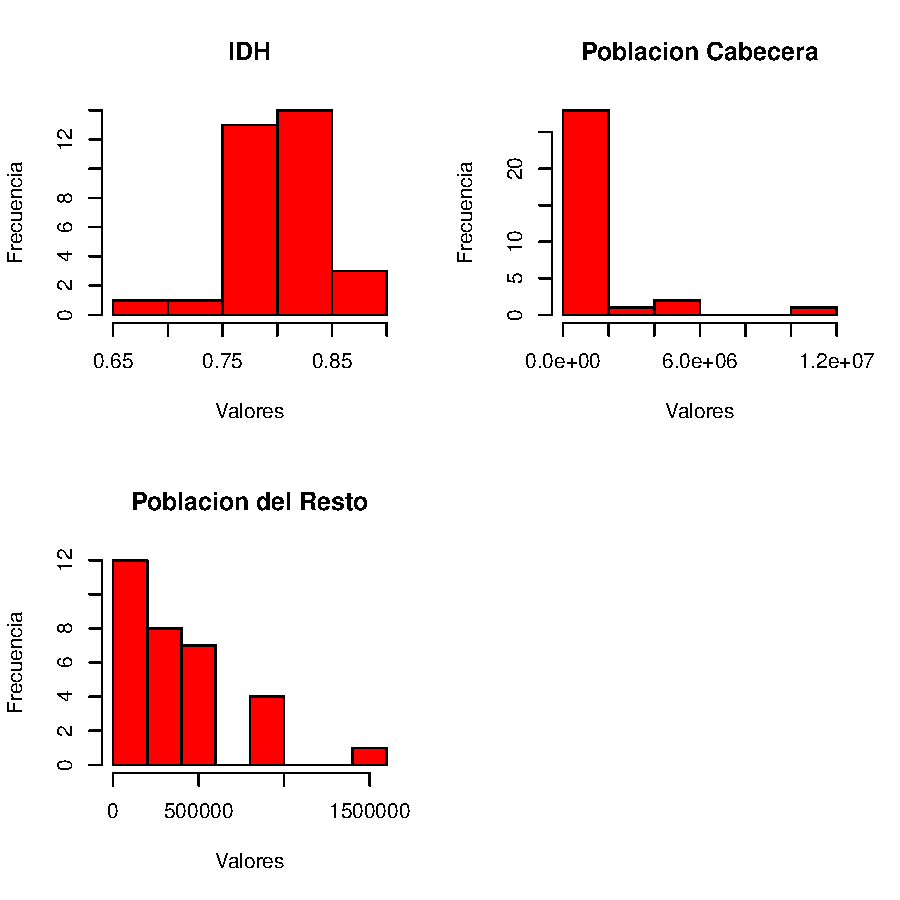
\includegraphics{Preliminar-hist1}
\caption{Distribuci<f3>n de Indicadores}
\label{hist1}
\end{figure}

Si quieren normalizar dado el sesgo de las poblaciones, se tranforma con logaritmo en case 10 y quedaria asi:

\begin{figure}[h]
\centering
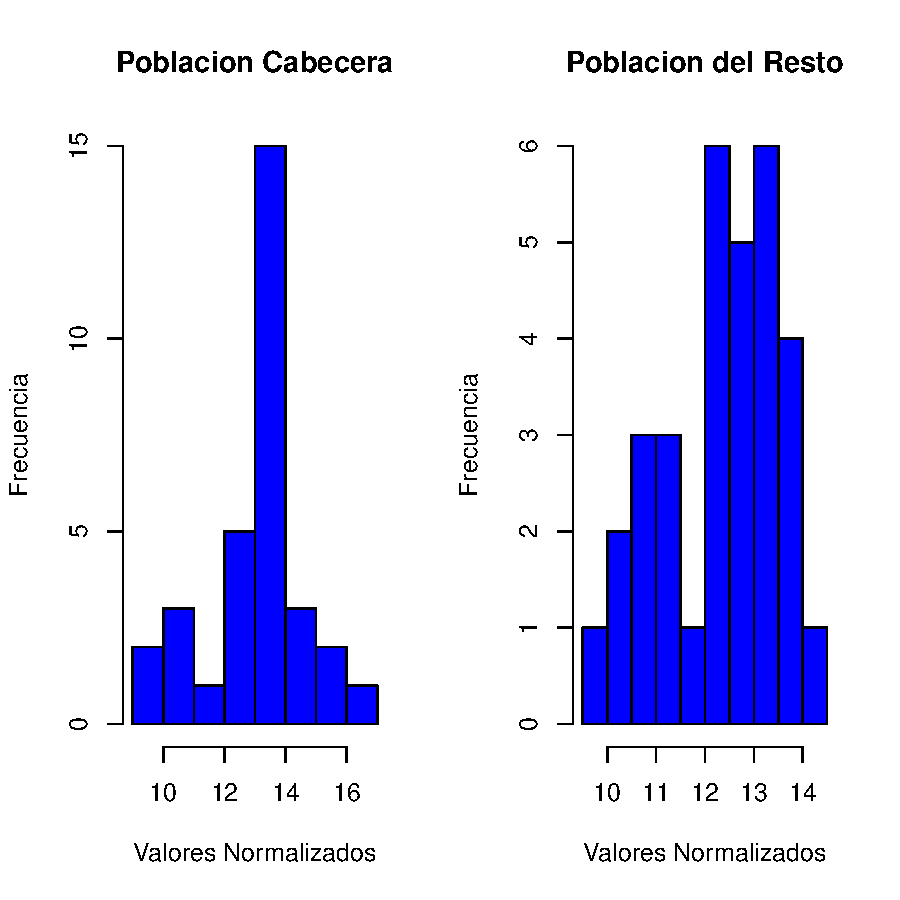
\includegraphics{Preliminar-hist}
\caption{Distribuci<f3>n de Indicadores de Poblaciones Normalizado}
\label{hist}
\end{figure}


\bibliographystyle{apalike}
\renewcommand{\refname}{Bibliografia}
\bibliography{Bibliografia}
\end{document}
